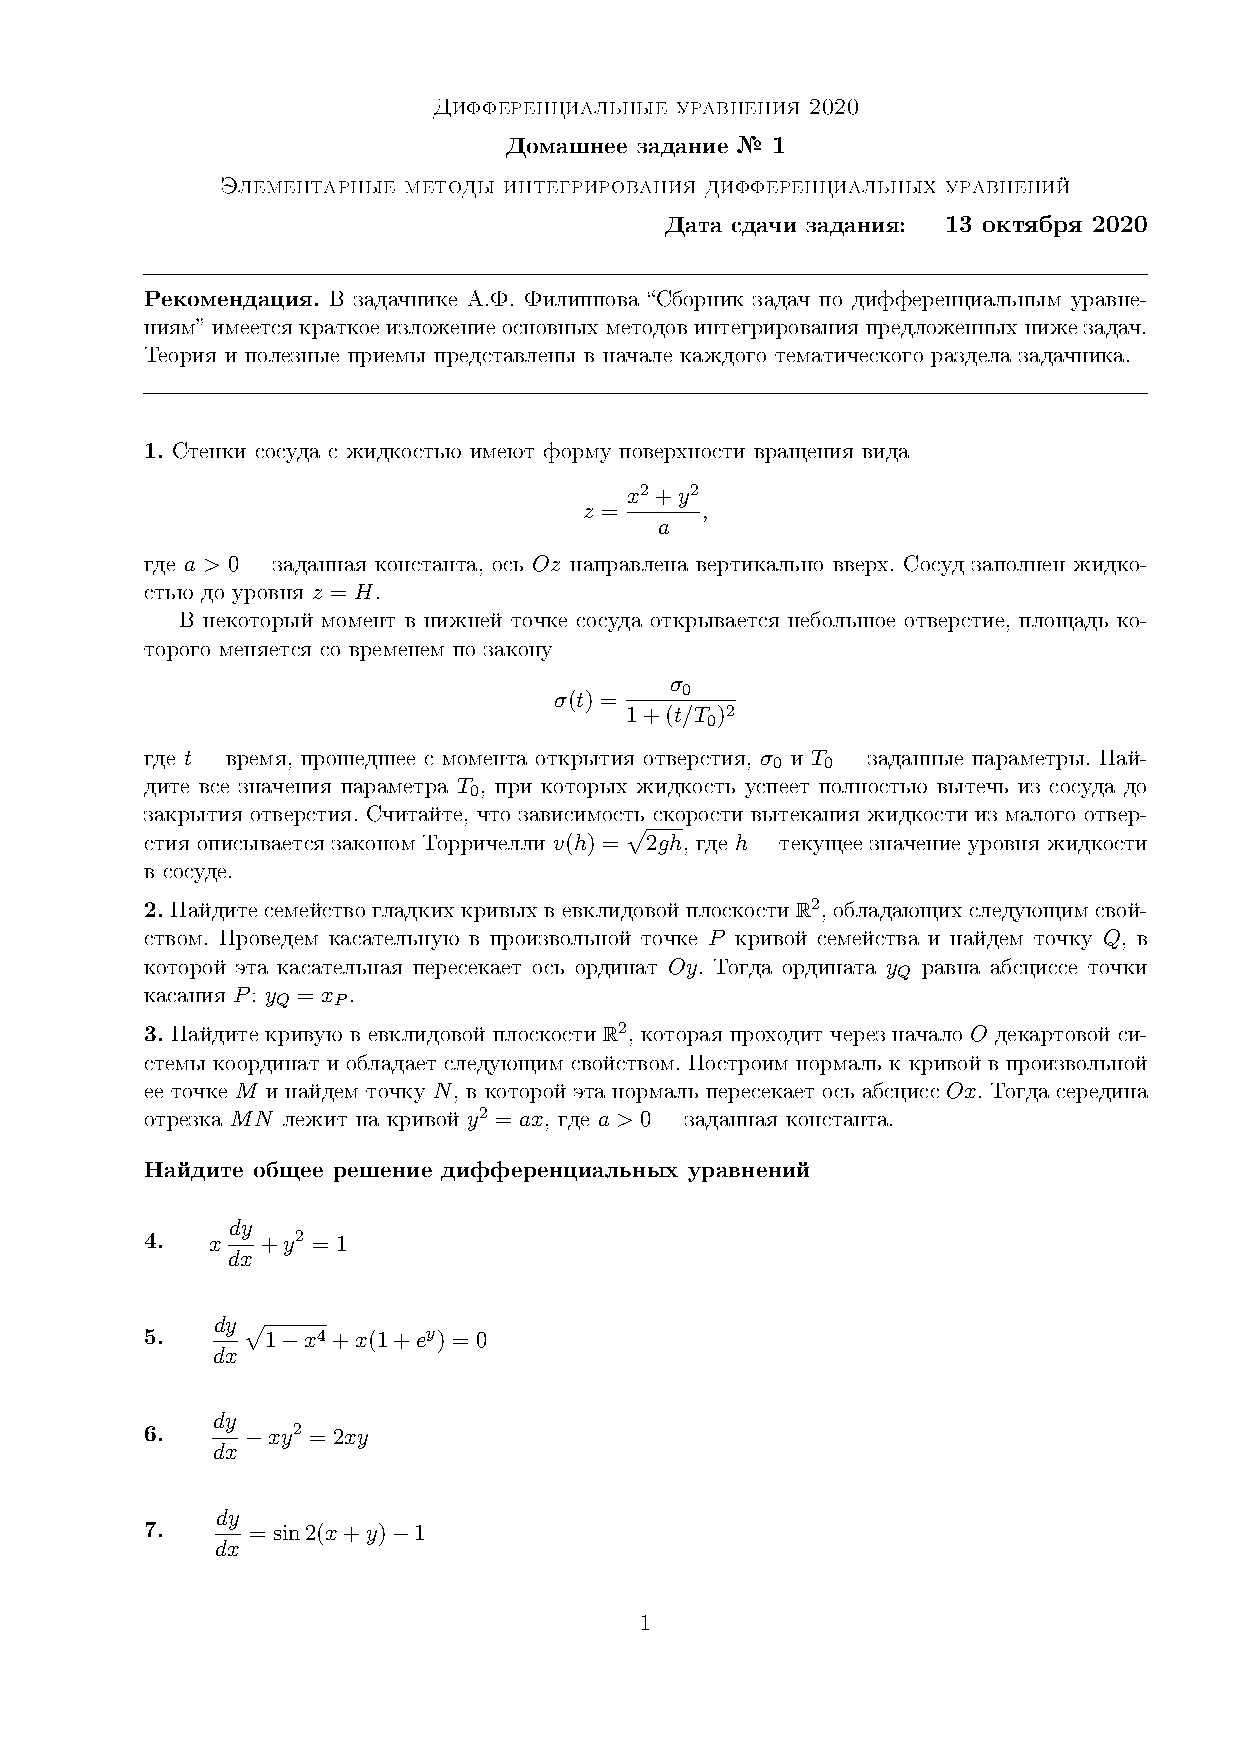
\includepdf[pages=1]{Tasks/HW-1-DE-2020}
\includepdf[pages=2]{Tasks/HW-1-DE-2020}
\newpage
\section*{Решения}
\subsection*{Задача 1}
Заметим, что
\begin{gather*}
	z = \frac{x^2 + y^2}{a}
	ah = x^2 + y^2\\
	\sqrt{ah} = r\\
	S = \pi r^2 = \pi ah
\end{gather*}
и
\begin{gather*}
	\sigma(t) = \frac{\sigma_0}{1 + \left(\frac{t}{T_0}\right)^2}
\end{gather*}
Тогда
\begin{gather*}
	\frac{\partial h}{\partial t} = \frac{- \sigma(t) v(h)}{ah} = - \frac{\sigma_0 T_0^2 \sqrt{2gh}}{(t^2 + T_0^2) \pi ah} = -C_1 \frac{1}{(t^2 + T_0^2)\sqrt{h}}\\
	C_1 = \frac{\sigma_0 T_0^2 \sqrt{2g}}{a \pi}\\
	\int\limits_{H}^{h(t)} \partial h = \int\limits_{0}^{t} -\frac{C_1}{t^2 + T_0^2} \partial t\\
	\frac{2}{3}(H^{\frac{3}{2}} - h(t)^{\frac{3}{2}}) = C_1 \frac{1}{T_0} \arctan \frac{t}{T_0}\\
	h(t) = (-\frac{3}{2} C_1 \frac{1}{T_0} \arctan \frac{t}{T_0} + H^{\frac{3}{2}})\frac{2}{3}\\
	h(t) = (-C_2 \arctan \frac{t}{T_0} + H^{\frac{3}{2}})^{\frac{2}{3}}\\
	C_2 = \frac{3}{2}\frac{1}{T_0}\frac{\sigma_0 T_0^2 \sqrt{2g}}{a \pi}\\
	t = T_0 \tan \frac{H^{\frac{3}{2}}}{C_2}\\
	\frac{H^{\frac{3}{2}}}{C_2} \in \left[0, \frac{\pi}{2}\right)\\
	\frac{H^{\frac{3}{2}}}{\frac{3}{2}\frac{1}{T_0}\frac{\sigma_0 T_0^2 \sqrt{2g}}{a \pi}} \in \left[0, \frac{\pi}{2}\right)\\
	T_0 > \frac{4a}{3 \sigma_0 \sqrt{2g}}
\end{gather*}

\subsection*{Задача 2}
Касательная задается уравнением $f(x) = y(x_0) + y'(x_0)(x - x_0)$, откуда $x_0 \frac{\partial y(x_0)}{\partial x} = y(x_0) - x_0$ и $x \frac{\partial y}{\partial x} = y - x$
\begin{gather*}
	y' - \frac{1}{x} y = -1\\
	c(x) + x c'(x) - c(x) = -1\\
	c'(x) = -\frac{1}{x}\\
	\int \partial c(x) = -\frac{1}{x} \partial x\\
	c(x) = -\ln|x| + c\\
	y = -x \ln|x| + cx
\end{gather*}

\subsection*{Задача 3}
\begin{gather*}
	f(x) = y(M_x) + y'(M_x)(x - M_x)\\
	f(x) = y'(M_x) x - M_x y'(M_x) + y(M_x)\\
	g(x) = kx + b\\
	k \cdot y'(M_x) = -1\\
	g(x) = -\frac{1}{y'(M_x)}(x - M_x) + y(M_x)\\
	g(N) = -\frac{1}{y'(M_x)}(N - M_x) + y(M_x) = 0\\
	N = M_x + yy'
\end{gather*}
Откуда
\begin{gather*}
	x = \frac{N + M_X}{2}\\
	y = \frac{M_y}{2}\\
	(\frac{M_y}{2})^2 = a \frac{N + M_x}{2}\\
	(\frac{M_y}{2})^2 = a (M_x + \frac{yy'}{2})\\
	y^2 = 2a(2x + yy')
\end{gather*}
Пусть $z = y^2$
\begin{gather*}
	z = 4ax + az'\\
	\frac{\partial z}{\partial x} - \frac{z}{a} = -4x\\
	\frac{\partial z}{z} = \frac{1}{a} \partial x\\
	\ln(z) = \frac{x}{a} + c\\
	z = e^{\frac{x}{a}}c\\
	\frac{1}{a} e^{\frac{x}{a}} c(x) + c'(x) e^{\frac{x}{a}} - \frac{e^{\frac{x}{a}} c(x)}{a} = -4x\\
	c'(x) = -\frac{4x}{e^{\frac{x}{a}}}\\
	c(x) = 4ae^{-\frac{x}{a}} (a+x) + c_0\\
	z = 4a(a+x) + c_0 e^{\frac{x}{a}}
\end{gather*}
Подставим точку $(0,3a)$ в уравнение
\begin{gather*}
	9a^2 = 4a^2 + c_0 e^{0}\\
	c_0 = 5a^2\\
	y^2 = 4a(a+x) + 5a^2 e^{\frac{x}{a}}
\end{gather*}

\subsection*{Задача 4}
\begin{gather*}
	x \frac{\partial y}{\partial x} + y^2 = 1\\
	\frac{\partial y}{\partial x} = \frac{1-y^2}{x}\\
	\frac{\partial y}{1-y^2} = \frac{\partial x}{x}\\
	\int \frac{\partial y}{1-y^2} \partial x = \int \frac{\partial x}{x}\\
	\frac{1}{2} \ln|1+y| - \frac{1}{2} \ln|1-y| = \ln |x| + c\\
	\frac{1+y}{1-y} = \pm x^2 c\\
	y = \frac{e^{2c}x^{2} \pm 1}{e^{2c}x^{2} \mp 1}\\
	y = \frac{c x^{2} \pm 1}{c x^{2} \mp 1}
\end{gather*}

\subsection*{Задача 5}
\begin{gather*}
	\frac{\partial y}{\partial x} \sqrt{1-x^4} + x(1+e^y)\\
	\frac{\partial y}{1 + e^{y}} = -\frac{x \partial x}{\sqrt{1-x^4}}\\
	\int \frac{\partial y}{1 + e^{y}} = \int -\frac{x \partial x}{\sqrt{1-x^4}}\\
	y - \ln(1+e^y) = \frac{1}{2} \arcsin(x^2) + c\\
	\frac{e^y}{1+e^y} = e^{\frac{1}{2} \arcsin(x^2)+c}
\end{gather*}

\subsection*{Задача 6}
\begin{gather*}
	\frac{\partial y}{\partial x} - xy^2 = 2xy\\
	\frac{\partial y}{\partial x} = x(y^2 + 2y)\\
	\frac{\partial y}{y^2+2y} = x \partial x\\
	\int \frac{\partial y}{y^2 + 2y} \partial x = \int x \partial x\\
	\frac{1}{2}\ln|y| - \frac{1}{2}\ln|y+2| = \frac{x^2}{2} + c\\
	y = \pm \frac{2e^{x^2+2c}}{e^{x^2+2c}-1}
\end{gather*}

\subsection*{Задача 7}
\begin{gather*}
	\frac{\partial y}{\partial x} = \sin(2(x+y)) - 1\\
	u = x+y\\
	\frac{\partial y}{\partial x} = \frac{\partial (u - x)}{\partial x} = \frac{\partial u}{\partial x} - 1\\
	\frac{\partial u}{\partial x} - 1 = u' - 1 = \sin(2u) - 1\\
	u' = \sin(2u)\\
	\frac{1}{2} \ln|\operatorname{ctg} u| = x + c\\
	\operatorname{ctg}(x+y) = \pm e^{2x}c\\
	x+y = \pm \operatorname{arcctg}(e^{2x}c) + \pi k\qquad k \in \mathbb{Z}\\
	y = \operatorname{arcctg}(e^{2x}c) - x + \pi k\qquad k \in \mathbb{Z}
\end{gather*}

\subsection*{Задача 8}
\begin{gather*}
	\frac{\partial y}{\partial x} = \frac{y+x}{y-x}\\
	u = y - x\\
	\frac{\partial y}{\partial x} = \frac{\partial (u + x)}{\partial x} = u' + 1\\
	\frac{\partial u}{\partial x} + 1 = \frac{2x + u}{u}\\
	\frac{\partial u}{\partial x} = \frac{2x}{u}\\
	\frac{1}{2}u^2 = x^2 + c\\
	(y - x)^2 = 2(x^2 + c)\\
	y = x \pm \sqrt{2x^2 + c}
\end{gather*}

\subsection*{Задача 9}
\begin{gather*}
	x \partial y - y \partial x = \sqrt{x^2+y^2} \partial x\\
	x \partial y = (\sqrt{x^2+y^2} + y) \partial x\\
	\frac{\partial y}{\partial x} = \frac{y + \sqrt{x^2+y^2}}{x}\\
	y = x u\\
	u + x \frac{\partial u}{\partial x} = u + \sqrt{1 + u^2}\\
	\frac{\partial x}{x} = \frac{\partial u}{\sqrt{1 + u^2}}\\
	\int \frac{\partial x}{x} \partial x = \int \frac{\partial u}{\sqrt{1 + u^2}} \partial x\\
	\ln (\sqrt{u^2 + 1} + u) = \ln|x| + c\\
	\sqrt{u^2 + 1} + u = xc\\
	\sqrt{x^2 + y^2} + y = cx^2\\
	y = \frac{x^2c^2 - 1}{2c}
\end{gather*}

\subsection*{Задача 10}
\begin{gather*}
	x \frac{\partial y}{\partial x} - y = x \tan \frac{y}{x}\\
	y = xu(x)\\
	x^{2} \frac{\partial u}{\partial x} + xu - xu = x \tan u\\
	x^{2} \frac{\partial u}{\partial x} = x \tan u\\
	\frac{\partial u}{\partial x} = \frac{\tan u}{x}\\
	\frac{\partial u}{\tan u} = \frac{\partial x}{x}\\
	\int \frac{\partial u}{\tan u} \partial x = \int \frac{\partial x}{x} \partial x\\
	\ln|\sin u| = \ln|x| + c\\
	|\sin u| = e^{c} x\\
	u = \pm \arcsin(e^{c} x)\\
	y = \pm x \arcsin(e^{c} x)\\
	y = \pm x \arcsin(c x)
\end{gather*}

\subsection*{Задача 11}
\begin{gather*}
	(1+x^2) \frac{\partial y}{\partial x} + xy = 1\\
	\frac{\partial y}{\partial x} + \frac{x}{1+x^2}y = \frac{1}{1+x^2}\\
	y' + a(x)y = b(x)\\
	y' + a(x)y = 0\\
	\int \frac{\partial y}{y} = \int - \frac{x}{1+x^2} \partial x\\
	\ln |y| = -\frac{1}{2} \ln|1+x^2| + c\\
	y = \frac{e^c}{\sqrt{1+x^2}} = \frac{c}{\sqrt{1+x^2}}\\
	\frac{\partial y}{\partial x} = \frac{\partial \frac{c}{\sqrt{1+x^2}}}{\partial x} = \frac{c'(x) \sqrt{1 + x^2} - c(x) \frac{2x}{2\sqrt{1+x^2}}}{1+x^2}\\
	c'(x) \sqrt{1+x^2} - \frac{xc(x)}{\sqrt{1+x^2}} + x \frac{c(x)}{\sqrt{1+x^2}} = 1\\
	c'(x) (1+x^2) - xc(x) + xc(x) = \sqrt{1+x^2}\\
	c'(x) = \frac{1}{\sqrt{1+x^2}}\\
	c(x) = \operatorname{arcsinh} x + c\\
	y = \frac{\operatorname{arcsinh}(x) + c}{\sqrt{1+x^2}}
\end{gather*}

\subsection*{Задача 12}
\begin{gather*}
	\frac{\partial s}{\partial t} + s \cos t = \frac{1}{2} \sin 2t\\
	s' + a(t)s = b(t)
	s' + a(t)s = 0\\
	\frac{\partial s}{\partial t} + s \cos t = 0\\
	\frac{\partial s}{s} = -\cos t \partial t\\
	s = c e^{-\sin t}\\
	\frac{\partial s}{\partial t} = \frac{\partial c(t) e^{-\sin t}}{\partial t} = c'(t) e^{-\sin t} - \cos t e^{-\sin t} c(t)\\
	c'(t)e^{-\sin t} - e^{-\sin t} c(t) \cos t + c(t) e^{-\sin t} \cos t = \frac{1}{2} \sin 2t\\
	c'(t) e^{-\sin t} = \sin t \cos t\\
	c(t) = e^{\sin t}(\sin t - 1) + c\\
	s = \sin t - 1 + c e^{-\sin t}
\end{gather*}

\subsection*{Задача 13}
\begin{gather*}
	\left(x \frac{\partial y}{\partial x} - 1\right) \ln x = 2y\\
	\frac{\partial y}{\partial x} - \frac{2y}{x \ln x} = \frac{1}{x}\\
	\frac{\partial y}{\ln^{2}x \partial x} - \frac{2y}{x \ln^{3} x} = \frac{1}{x \ln^{2} x}\\
	\frac{\partial y}{\ln^{2}x \partial x} - \frac{\partial }{\partial x}\frac{1}{\ln^{2} x} = \frac{1}{x \ln^{2} x}\\
	\frac{\partial }{\partial x} \frac{y}{\ln^2 x} = \frac{1}{x \ln^{2} x}\\
	\int \frac{\partial }{\partial x} \frac{y}{\ln^2 x} \partial = \int \frac{1}{x \ln^{2}} \partial x\\
	\frac{y}{\ln^2 x} = -\frac{1}{\ln^{2} x} +c\\
	y = \ln x (c \ln x -1)
\end{gather*}

\subsection*{Задача 14}
\begin{gather*}
	xy(1+xy^2) \frac{\partial y}{\partial x} = 1\\
	\frac{\partial x}{\partial y} = xy(1+xy^2)\\
	u = \frac{1}{x}\\
	-\frac{1}{u^2}\frac{\partial u}{\partial y} = \frac{y}{u}(1+\frac{y^2}{u})\\
	\frac{\partial u}{\partial y} + uy + y^3 = 0\\
	\frac{\partial u}{\partial y} + uy = 0\\
	\ln u = -\frac{1}{2}y^2 + c\\
	u = e^{\frac{1}{2}y^2} c\\
	c'(y) e^{-\frac{1}{2}y^2} - y c(y) e^{-\frac{1}{2}y^2} + yc(y) e^{-\frac{1}{2}y^2} = -y^3\\
	c'(y) = -y^3 e^{\frac{1}{2}y^2}\\
	c(y) = -e^{\frac{1}{2}y^2}(y^2 - 2) + c\\
	u = -(y^2 - 2) + e^{-\frac{1}{2}y^2}c\\
	x = \left(-(y^2 - 2) + e^{-\frac{1}{2}y^2}c\right)^{-1}
\end{gather*}

\subsection*{Задача 15}
\begin{gather*}
	x \frac{\partial y}{\partial x} - y = x^2 \sqrt{y}\\
	\frac{\partial y}{\partial x} = x\sqrt{y} + \frac{y}{x}\\
	u = \sqrt{y}\\
	2u \frac{\partial u}{\partial x} = x u + \frac{u^2}{x}\\
	2\frac{\partial u}{\partial x} = x + \frac{u}{x}\\
	\frac{1}{\sqrt{x}} c(x) + 2\sqrt{x}c'(x) - \frac{c(x)}{\sqrt{x}} = x\\
	c'(x) = \frac{x}{2\sqrt{x}}\\
	c(x) = \frac{x^{\frac{3}{2}}}{3} + c\\
	u = \frac{x^2}{2} + c x^{\frac{1}{2}}\\
	y = \left(\frac{x^2}{3} + c x^{\frac{1}{2}}\right)^2
\end{gather*}

\subsection*{Задача 16}
\begin{gather*}
	(x^2 + y^{\alpha}) \partial x + (\alpha x - 2y) \partial y = 0\\
	\frac{\alpha x - 2y}{\partial x} = \frac{x^2 + y^\alpha}{\partial y}\\
	\alpha = \alpha y^{\alpha - 1}
\end{gather*}
\begin{enumerate}
	\item[$\alpha = 1$] 
		\begin{gather*}
			(x^2 + y) \partial x + (x - 2y) \partial y = 0\\
			\frac{\partial U}{\partial x} = x^2 + y\\
			\int (x^2 + y) \partial x = \frac{1}{3} x^3 + f_1(y) + c\\
			\frac{\partial U}{\partial y} = x - 2y\\
			\int (x - 2y) \partial y = f_2(x) - y^2 + c\\
			U(x,y) = \frac{1}{3}x^3 - y^2 + yx + c\\
			\frac{1}{3}x^3 - y^2 + yx + c = 0
		\end{gather*}
	\item[$\alpha = 0$]
		\begin{gather*}
			\frac{\partial U}{\partial y} = -2y\\
			\frac{\partial U}{\partial x} = x^2 + 1\\
			U(x,y) = \int(x^2+1) \partial x = \frac{1}{3} x^3 + x + c + f_y(y)\\
			U(x,y) = \int(-2y) \partial y = -y^2 + c + f_x(x)\\
			U(x,y) = \frac{1}{3} x^3 + x - y^2 + c\\
			\frac{1}{3} x^3 + x - y^2 + c = 0
		\end{gather*}
\end{enumerate}


\subsection*{Задача 17}
\begin{gather*}
	(\cos^2(x) - (x+y)\sin\frac{x}{\alpha}) \partial x + 2(\alpha - 1) \sin^2(x) \partial y = 0\\
	\frac{\partial (\cos^2(x) - (x+y)\sin\frac{x}{\alpha})}{\partial y} = -\sin\frac{x}{\alpha}\\
	\frac{\partial (2(2\alpha-1)\sin^2 x)}{\partial x} = 4 \sin x \cos x (\alpha - 1) = 2(\alpha - 1) \sin(2x)\\
	2(\alpha - 1)\sin(2x) + \sin \frac{x}{\alpha} = 0
\end{gather*}
\begin{enumerate}
	\item[$\alpha = \frac{1}{2}$]
	\begin{gather*}
		\sin(2x) - \sin(2x) = 0\\
		0 = 0
	\end{gather*}
	\vskip 0.1in
	\begin{gather*}
		\frac{\partial U}{\partial x} = \cos^2(x) - (x+y) \sin(2x)\\
		\frac{\partial U}{\partial y} = -\sin^2(x)\\
		U = -y \sin^2 x + f(x)\\
		\frac{\partial U}{\partial x} = -2y\sin(x)\cos(x) + f'(x) = -y\sin(2x) + \cos^2(x) - x\sin(2x)\\
		U = x \cos^2 x - y\sin^2 x = c
	\end{gather*}
\end{enumerate}


\subsection*{Задача 18}
\begin{gather*}
	\left(\frac{1}{x} - \frac{y^{\alpha}}{(x-y)^2}\right) \partial x - \left(\frac{1}{y} - \frac{x^\alpha}{(x-y)^2}\right) \partial y = 0\\
	\left(\frac{1}{x} - \frac{y^{\alpha}}{(x-y)^2}\right) \partial x + \left(-\frac{1}{y} + \frac{x^\alpha}{(x-y)^2}\right) \partial y = 0\\
	\frac{\partial \left(\frac{1}{x} - \frac{y^{\alpha}}{(x-y)^2}\right)}{\partial y} = \frac{\alpha y^{\alpha - 1}(x-y)^2 - 2(x-y)y^{\alpha}}{(x-y)^4} = \frac{-\alpha y^{\alpha - 1}(x-y) - 2y^{\alpha}}{(x-y)^3}\\
	\frac{\partial \left(-\frac{1}{y} + \frac{x^\alpha}{(x-y)^2}\right)}{\partial x} = \frac{\alpha x^{\alpha-1}(x-y)^2 - 2(x-y)x^{\alpha}}{(x-y)^4} = \frac{\alpha x^{\alpha-1}(x-y) - 2x^{\alpha}}{(x-y)^3}\\
	\alpha(x-y)(x^{\alpha - 1} + y^{\alpha - 1}) - 2(x^{\alpha} - y^{\alpha}) = 0\\
\end{gather*}
\begin{enumerate}
\item[$\alpha = 2$]
	\begin{gather*}
		\alpha(x-y)(x^{\alpha - 1} + y^{\alpha - 1}) - 2(x^{\alpha} - y^{\alpha}) = 0\\
		2(x-y)(x^{2 - 1} + y^{2 - 1}) - 2(x^{2} - y^{2}) = 0\\
		2(x^{2} - y^{2}) - 2(x^{2} - y^{2}) = 0\\
		0 = 0
	\end{gather*}
\item[$\alpha = 0$]
	\begin{gather*}
		\frac{\partial U}{\partial x} = \frac{1}{x} - \frac{y^2}{(x-y)^2}\\
		\frac{\partial U}{\partial x} = -\frac{1}{y} + \frac{x^2}{(x-y)^2}\\
		U = \int \frac{\partial U}{\partial x} \partial x = \ln|x| + \frac{y^2}{x-y} + f_y(y)\\
		\frac{2y(x-y)}{(x-y)^2} + f_y'(y) = -\frac{1}{y} + \frac{x^2}{(x-y)^2}\\
		f_y'(y) = 1 - \frac{1}{y}\\
		f_y(y) = -\ln|y| + y + c\\
		U = \ln|x| - \ln|y| + \frac{xy}{x-y} + c\\
		\ln|x| - \ln|y| + \frac{xy}{x-y} = c
	\end{gather*}
\end{enumerate}


\subsection*{Задача 19}
\begin{gather*}
	\left(1 + \frac{3y^2}{x^2}\right) \partial x = \frac{2y}{x} \partial y\\
	\frac{\partial M}{\partial y} = \frac{\partial (1 + \frac{3y^2}{x^2})}{\partial y} = \frac{6y}{x^2}\\
	\frac{\partial N}{\partial x} = \frac{\partial (\frac{2y}{x})}{\partial x} = -\frac{2y}{x^2}\\
	\mu \frac{6y}{x^2} = \mu \frac{2y}{x^2}\\
	-\mu_x \frac{2y}{x} + \frac{2y}{x} \mu = \mu_y (1+ \frac{3y^2}{x^2}) + \frac{6y}{x^2} \mu\\
	-\mu_x \frac{2y}{x} - \mu_y (1+\frac{3y^2}{x^2}) = \mu \frac{4y}{x^2}\\
	\mu = -\frac{1}{x^2}\qquad \mu_x = \frac{2}{x^3}\\
	(-\frac{1}{x^2}(1+\frac{3y^2}{x^2})) \partial x + \frac{2}{x^5} \partial y = 0\\
	\frac{\partial U}{\partial x} = -\frac{1}{x^2} - \frac{3y^2}{x^4}\\
	\frac{\partial U}{\partial y} = \frac{2y}{x^3}\\
	U = \int \frac{\partial U}{\partial y} \partial y = \frac{y^2}{x^3} + f(x)\\
	\frac{\partial U}{\partial x} = -\frac{3y^2}{x^4} + f'(x) = -\frac{1}{x^2} - \frac{3y^2}{x^4}\\
	f'(x) = -\frac{1}{x^2}\\
	f(x) = \frac{1}{x} + c\\
	U = \frac{y^2}{x^3} + \frac{1}{x} + c\\
	\frac{y^2}{x^3} + \frac{1}{x} + c = 0
\end{gather*}


\subsection*{Задача 20}
\begin{gather*}
	(2x + \frac{y}{2x}) \partial x + (x^2 - \frac{y+1}{x}) \partial y = 0\\
	\frac{\partial M}{\partial y} = \frac{\partial (2x + \frac{y}{x^2})}{\partial y} = \frac{1}{x^2}\\
	\frac{\partial N}{\partial x} = \frac{\partial (x^2 - \frac{y+1}{x})}{\partial x} = 2x + \frac{y+1}{x^2}\\
	\mu_y (2x + \frac{y}{x^2}) + \frac{1}{x^2} \mu = \mu_x (x^2 - \frac{y+1}{x}) + (2x + \frac{y+1}{x^2})\mu\\
	\mu(2x + \frac{y}{x^2}) = \mu_x (\frac{y+1}{x} - x^2) + \mu_y (2x + \frac{y}{x^2})\\
	\frac{\partial U}{\partial x} = 2xe^y + \frac{y}{x^2}e^{y}\\
	\frac{\partial U}{\partial y} = x^2e^{y} - \frac{y+1}{x} e^{y}\\
	U = \int \frac{\partial U}{\partial x} \partial x = x^2 e^y - \frac{y}{x}e^y + f(y)\\
	\frac{\partial U}{\partial y} = x^2e^y - \frac{e^y}{x} - \frac{y}{x}e^{y} + f'(y) = x^2e^{y} - \frac{y+1}{x} e^y\\
	f'(y) = 0\qquad f(y) = c\\
	U = x^2e^{y} - \frac{y}{x} e^{y} = c\\
	x^2e^{y} - \frac{y}{x} e^{y} = c
\end{gather*}


\subsection*{Задача 21}
\begin{gather*}
	\ln y \partial x - \frac{x}{y} \partial y = 0\\
	\frac{\partial \ln y}{\partial y} = \frac{1}{y}\\
	\frac{-\partial \frac{x}{y}}{\partial y} = -\frac{1}{y}\\
	\mu_x (-\frac{x}{y}) - \frac{1}{y} \mu = \mu_y \ln y + \frac{1}{y}\mu\\
	\frac{2}{y} \mu = -\frac{x}{y} \mu_x - \ln y \mu_y\\
	\mu = \frac{1}{x^2}\\
	\frac{1}{x^2} \ln y \partial x - \frac{1}{xy} \partial y = 0\\
	\frac{\partial U}{\partial x} \partial x = -\frac{1}{x} \ln y + f(y)\\
	\frac{\partial U}{\partial y} = -\frac{1}{xy} + f'(y) = -\frac{1}{xy}\\
	f'(y) = 0\\
	f(y) = c\\
	U = -\frac{1}{x} \ln y + c\\
	-\frac{1}{x} \ln y + c = 0
\end{gather*}
